\documentclass[MathsNotesBase.tex]{subfiles}



\date{\vspace{-6ex}}


\begin{document}
\searchableSubsection{\chapterTitle{Vector Spaces}}{vector spaces, polynomials, periodic functions}{\bigskip\bigskip}

\searchableSubsection{\sectionTitle{Vector Space properties}}{vector spaces, polynomials}{\bigskip}
	
	\bigskip
	\searchableSubsection{Definition of a Vector Space}{vector spaces}{\bigskip
	
		\paragraph*{A field} $F$ is a subfield of $\mathbb{C}$ if the following properties hold:
		\begin{itemize}
		\item If $a, b \in F$, then $a + b \in F$.
		\item If $a \in F$, then $-a \in F$.
		\item If $a, b \in F$, then $ab \in F$.
		\item If $a \in F \text{ and } a \ne 0$, then $a^{-1} \in F$.
		\item $1 \in F$.
		\end{itemize}
		
		Note that using the first, second and last of these axioms we can deduce that $1 - 1 = 0$ is an element of $F$.\\
		
		\bigskip	
		Let $F$ denote a field which is a subfield of $\mathbb{C}$ and $V$ denote a vector space over $F$.
		\begin{definition}
		\textbf{Addition, Scalar Multiplication}
		\begin{itemize}
		\item{An \textbf{addition} on a set $V$ is a function that assigns an element $u + v \in V$ to each pair of elements $u, v \in V$.}
		\item{A \textbf{scalar multiplication} on a set $V$ is a function that assigns an element $\lambda{v} \in V$ to each $\lambda \in F$ and each $v \in V$.}
		\end{itemize}
		Note that both functions are closed over $V$.
		\end{definition}	
		\begin{definition}
		\textbf{A vector space} is a set $V$ along with an addition on $V$ and a scalar multiplication on $V$ such that the following properties hold:
		\paragraph*{commutativity} $\u + \v = \v + \u$ for all $\u, \v \in V$;
		\paragraph*{associativity} $(\u + \v) + \w = \u + (\v + \w)$ and $(ab)\v = a(b\v)$ for all $\u, \v, \w \in V$ and all $a, b \in F$;
		\paragraph*{additive identity} there exists an element $\0 \in V$ such that $\v + \0 = \v$ for all $\v \in V$;
		\paragraph*{additive inverse} for every $\v \in V$ there exists $\w \in V$ such that $\v + \w = \0$;
		\paragraph*{multiplicative identity} $1\v = \v$ for all $\v \in V$;
		\paragraph*{distributive properties} $a(\u + \v) = a\u + a\v$ and $(a + b)\u = a\u + b\u$ for all $a, b \in F$ and $\u,\v \in V$;
		\end{definition}
	}
	
	\bigskip\bigskip
	\searchableSubsection{Derived properties of a Vector Space}{vector spaces}{\bigskip


		\labeledProposition{A vector space contains a unique additive identity element.}{unique_additive_identity}
		\begin{proof}
		If $\V{0'}$ is also an additive identity then by the additive identity property, 
		\[ \V{0} + \V{0'} = \V{0} \]
		but since $\V{0}$ is also an additive identity,
		\[ \V{0'} + \V{0} = \V{0'} \]
		Then, by the commutativity of vector addition,
		\[ \V{0} = \V{0} + \V{0'} = \V{0'} + \V{0} = \V{0'} \qedhere \]
		\end{proof}
		
	
		\labeledProposition{A vector space contains a unique additive inverse for each element.}{unique_additive_inverse}
		\begin{proof}
		If $\v$ and $\w$ are both additive inverses of $\u$ then, by the additive inverse property we have,
		\[ \u + \v = \0 \text{ and also } \u + \w = \0 \]
		using the uniqueness of the additive identity,
		\[ \u + \v = \0 = \u + \w \]
		Then, if we add one of the additive inverses of $\u$ to both sides,
		\[ \u + \v + \v = \u + \w + \v \]
		and use the associativity of vector addition,
		\begin{align*}
		(\u + \v) + \v &= (\u + \v) + \w \\
		\0 + \v &= \0 + \w \\
		 \v &= \w \qedhere
		\end{align*}
		\end{proof}
		Because additive inverses are unique we can use the notation $-\v$ to denote the additive inverse of $\v$. Then we define $\w - \v$ to mean $\w + -\v$.
		\begin{definition}{Vector Subtraction}
		\[ \u - \v \coloneqq \u + -\v \]
		\end{definition}
		
	
		\labeledProposition{$0\v = \0$ for every $\v \in V$.}{multiplication_by_zero}
		Note that this proposition is asserting something about scalar multiplication and the additive identity of $V$. The only part of the definition of a vector space that connects scalar multiplication and vector addition is the distributive property. Therefore the distributive property must be used in this proof.
		\begin{proof}
		Firstly take,
		\[ \v + 0\v = 0\v + 1\v \]
		and then use the properties of the underlying field to say
		\[ (0 + 1)\v = 1\v = \v \]
		Now we have shown that,
		\[ \v + 0\v = \v \]
		which, by the definition and uniqueness of the additive identity, shows that $0\v = \0$. But if we want to continue algebraically we can now add the additive inverse to both sides,
		\[ (\v + -\v) + 0\v = (\v + -\v) \]
		\[ \0 + 0\v = 0\v = \0 \qedhere\]
		\end{proof}
		Another, simpler proof exists. 
		\begin{proof}
		Using the underlying field properties and the distributivity of scalar vector multiplication,
		\[ 0\v = (0 + 0)\v = 0\v + 0\v \]
		and then adding the additive inverse to both sides,
		\begin{align*}
		(0\v + -(0\v)) &= (0\v + -(0\v)) + 0\v \\
		\0 &= \0 + 0\v = 0\v \qedhere
		\end{align*}
		\end{proof}
		
	
		\labeledProposition{$a\0 = \0$ for every $a \in F$.}{multiplication_of_zero}
		\begin{proof}
		Using the distributivity of scalar multiplication of vectors and the additive identity,
		\[ a\0 = a(\0 + \0) = a\0 + a\0 \]
		Then, adding the additive inverse to both sides,
		\begin{align*}
		(a\0 + -(a\0)) &= a\0 + (a\0 + -(a\0))\\
		\0 &= a\0 + \0 = a\0 \qedhere
		\end{align*}
		\end{proof}
		
	
		\labeledProposition{$(-1)\v = -\v$ for every $\v \in V$.}{multiplication_by_minus_one}
		\begin{proof}
		Using the distributivity of scalar multiplication of vectors and the underlying field properties we have,
		\[ (-1)\v + \v = (-1)\v + 1\v = (-1 + 1)\v = 0\v = \0 \]
		Now we could add the additive inverse to both sides to show that,
		\begin{align*} 
		(-1)\v + (\v + -\v) &= \0 + -\v \\
		(-1)\v + \0 &= \0 + -\v \\
		(-1)\v &= \v \qedhere
		\end{align*}
		But we already have,
		\[ (-1)\v + \v =\0 \]
		and this, by the definition of the additive inverse, proves that $(-1)\v$ is an additive inverse of $\v$. Since we have previously proven the uniqueness of the additive inverse in \autoref{prop:unique_additive_inverse} we can conclude, in fact, that $(-1)\v = -\v$ the unique additive inverse of $v$.
		\end{proof}
	}
	
	\bigskip
	\searchableSubsection{The notation $F^S$}{vector spaces}{\bigskip
	If $S$ is a set then $F^S$ denotes the set of functions $S \mapsto F$.\\
	\paragraph{Addition} is defined as, for $f, g, (f + g) \in F^S$,
		\[ (f + g)(x) = f(x) + g(x) \]
	for all $x \in S$.
	\paragraph{Scalar multiplication} is defined as, for $\lambda \in F, \lambda{f} \in F^S$,
		\[ (\lambda{f})(x) = \lambda{f}(x) \]
	for all $x \in S$.
	\paragraph{Example:} If $S$ is the interval $[0,1]$ and $F = \R{}$ then $\R{[0,1]}$ is the set of real-valued functions on the interval $[0,1]$. $\R{[0,1]}$ is a vector space with additive identity $0: [0,1] \mapsto \R{}$ defined as $0(x) = 0$ and the additive inverse of some function $f \in \R{[0,1]}$ is the function defined as $(-f)(x) = -f(x)$.\\
	Any \emph{non-empty} set $S$ in conjunction with a subset of $\C{}$ would similarly produce a vector space. In fact, the vector space $F^n$ can be thought of as the space of functions from the set $\{1, 2, 3,\dots,n \}$ to F. For example, vectors in 3-dimensional space can be viewed as:
	\begin{align*}
	\begin{bmatrix} 
		x \\
		y \\
		z \\
	\end{bmatrix}
	\equiv f: \{1, 2, 3\} \mapsto \R{} \text{ with } f(t) =
	\begin{cases} 
	   x & t = 1 \\
	   y & t = 2 \\
	   z & t = 3
	\end{cases}
	\end{align*}
	}
	
	\bigskip
	\searchableSubsection{Polynomials as a vector space}{vector spaces, polynomials}{\bigskip 		
	\label{ssection:polynomials_as_vector_spaces}
		A very important example involves treating a polynomial as a vector. A function $p: F \mapsto F$ is called a polynomial with coefficients in $F$ if there exist $a_0,\dots,a_m \in F$ such that,
		\[ p(z) = a_0 + a_1z + a_2z^2 + \dots + a_mz^m \]
		for all $z \in F$.\\
		Then we can define a vector space, $P(F)$, to be the set of all polynomials with coefficients in $F$.
		\paragraph*{Addition} on $P(F)$ is defined as,
		\[ (p + q)(z) = p(z) + q(z) \hspace{20pt}\text{ for } p,q \in P(F), z \in F \]
		whose associativity is clear from the definition and the commutativity can be shown by,
		\begin{align*}
		( (p + q) + r )(z) &= (p + q)(z) + r(z) \\
		  &= p(z) + q(z) + r(z) \\
		  &= p(z) + (q + r)(z) \\
		  &= ( p + (q + r) )(z)
		\end{align*}
		\paragraph*{Scalar multiplication} on $P(F)$ is defined as,
		\[ (ap)(z) = ap(z) \hspace{20pt}\text{ for } p \in P(F), a,z \in F  \]
		whose associativity can be shown by substituting $(ab)$ for $a$ in the definition,
		\[ [(ab)p](z) = (ab)p(z) \]
		Then, by the associativity of the multiplication of the elements of the field $F$ we have,
		\[ (ab)p(z) = a[b(p(z)] \]
		then we use the definition in reverse,
		\[ a[b(p(z)]) = a[(bp)(z)] = [a(bp)](z) \]
		(compare with $(ab)\v = a(b\v)$)
		\paragraph*{modeling}Concretely, each $p(z) \in P(F)$ is a vector that could be modeled, say, as
		\[ \V{p} = \{\, (a_0,a_1,\dots,a_m) \mid p(z) = a_0 + a_1z + a_2z^2 + \dots + a_mz^m \in P(F)\, \} \]
	}


\searchableSubsection{\sectionTitle{Subspaces of vector spaces}}{vector spaces, polynomials, periodic functions}{\bigskip}

	\bigskip		
	\searchableSubsection{Definition of a Subspace}{vector spaces}{\bigskip
		\begin{definition}
		A set $U$ is a subspace of $V$ if it is a subset of $V$ and if the same addition and multiplication over $U$ forms a vector space.
		\end{definition}
		Considering the required properties of a vector space, we can see that commutativity and associativity of the addition; associativity of the scalar multiplication; and distributivity of the scalar multiplication over the addition; will all be satisfied as we have the same addition and multiplication over a subset of the elements in $V$. That's to say, the vector space properties ensure that these properties hold $\forall \v \in V$ and we have $\forall \u \in U, \u \in V$. \\Furthermore, the multiplicative identity also holds $\forall \v \in V$ so will also hold for every element of $U$.
		\paragraph*{So what remains to be proven to satisfy the requirements of a subspace?}
		\begin{itemize}
		\item{Existence of the additive identity}
		\item{Existence of an additive inverse for every element of $U$}
		\item{Closure of the addition and scalar multiplication over $U$}
		\end{itemize}
		Note, however that - having proved in \autoref{prop:multiplication_by_minus_one} that multiplication by $-1$ gives the additive inverse - closure of the scalar multiplication over $U$ also implies the presence in $U$ of the additive inverse of every element of $U$. So, actually, what we need to prove for $U$ to be a subspace is only,
		\begin{itemize}
		\item{$\0 \in U$}
		\item{Closure of the addition and scalar multiplication over $U$}
		\end{itemize}
	}
	
	\searchableSubsection{A subspace of the polynomials}{vector spaces, polynomials}{\bigskip

		An example of a subspace of the polynomials, $P(F)$ is,
		\[ \setc*{p \in P(F)}{p(3) = 0} \]
		Members of this subspace include:
		\begin{itemize}
		\item{$p(z) = 3 - z$}
		\item{$p(z) = 9 - z^2$}
		\item{$p(z) = 3 - z + 3z^2 - z^3$}
		\item{$p(z) = 12z - 4z^2$}
		\item{\dots etc.}
		\end{itemize}
		To verify this we need to show that addition and multiplication are closed over this set and that $\0$ is a member of the set. It's easy to see that $\0$ is a member of the set as,
		\[ p(3) = 0 + 0(3) + 0(3)^2 + \dots + 0(3)^m = 0 \]
		as required. Scalar multiplication is closed as,
		\[ ap(3) = a(0) = 0 \]
		whereas addition can be shown to be closed as,
		\[ (q + r)(3) = q(3) + r(3) = 0 + 0 = 0 \]
		Note that for values of $z \ne 3$, the closure of these functions is the same as for the general case of $P(F)$.
	}
	
	\bigskip\bigskip
	\searchableSubsection{Sums and Direct Sums}{vector spaces}{\bigskip\bigskip
		\begin{definition}
		If $U_1,U_2,\dots,U_m$ are subspaces of $V$ then their sum is defined as
		\[ U_1 + U_2 + \dots + U_m = \left\{\,\V{u_1} + \V{u_2} + \dots + \V{u_m} \,\mid\, \V{u_1} \in U_1, \V{u_2} \in U_2, \dots , \V{u_m} \in U_m\,\right\} \]
		\end{definition}
		The sum of the subspaces of $V$ is also a subspace of $V$ because,
		\begin{itemize}
		\item{Closure of addition
			\begin{align*} 
			&(\V{u_1} + \V{u_2} + \dots + \V{u_m}) + (\V{u_1'} + \V{u_2'} + \dots + \V{u_m'}) \\
			=\, &(\V{u_1} + \V{u_1'}) + (\V{u_2} + \V{u_2'}) + \dots + (\V{u_m} + \V{u_m'}) \\
			=\, &\V{v_1} + \V{v_2} + \dots + \V{v_m} \hspace*{40pt} \text{where } \V{v_1} \in U_1, \V{v_2} \in U_2, \dots , \V{v_m} \in U_m
			\end{align*}
		}
		\item{Closure of scalar multiplication
				\begin{align*} 
				&a(\V{u_1} + \V{u_2} + \dots + \V{u_m}) \hspace*{40pt} \text{where } a \in F\\
				=\, &a\V{u_1} + a\V{u_2} + \dots + a\V{u_m} \\
				=\, &\V{v_1} + \V{v_2} + \dots + \V{v_m} \hspace*{40pt} \text{where } \V{v_1} \in U_1, \V{v_2} \in U_2, \dots , \V{v_m} \in U_m
				\end{align*}
		}
		\item{Existence of $\0$
			\begin{align*}
			&U_1,U_2,\dots,U_m \text{ are subspaces } \\
			\implies &\0 \in U_1, \0 \in U_2,\dots,\0 \in U_m \\
			\implies &\0 + \0 + \dots + \0 \in U_1 + U_2 + \dots + U_m
			\end{align*}
			Note though, that this may not be the only way of producing $\0$ from the sum of vectors of these subspaces. That's to say, there could be some $(\V{u_1} + \V{u_2} + \dots + \V{u_m}) = \0$ and this is a key difference from direct sums.
		}
		\end{itemize}

		\bigskip
		\labeledProposition{$U_1 + U_2 + \dots + U_m$ is the smallest subspace of $V$ containing $U_1,U_2,\dots,U_m$.}{sum_smallest_subspace}
		\begin{proof}
		\begin{itemize}[label={}]
		\item{$U_1 + U_2 + \dots + U_m$ is a subspace of $V$ that contains $U_1,U_2,\dots,U_m$ because we can obtain $U_i$ by setting all the $u_j$ for $j \neq i$ to $\0$.}
		\item{If a subspace of $V$ contains $U_1,U_2,\dots,U_m$ then, by the closure of addition, it must also contain $U_1 + U_2 + \dots + U_m$.}
		\item{Therefore the smallest subspace of $V$ that contains $U_1,U_2,\dots,U_m$ is $U_1 + U_2 + \dots + U_m. \qedhere$}
		\end{itemize}
		\end{proof}
		
		\bigskip
		\begin{definition}
		If $U_1,U_2,\dots,U_m$ are subspaces of $V$ then their \textbf{direct sum} is defined as,
		\[ \textstyle{U_1 \oplus U_2 \oplus \dots \oplus U_m} =  \setc*{ \V{u_1} + \V{u_2} + \dots + \V{u_m} }{ \V{u_1} \in U_1, \V{u_2} \in U_2, \dots , \V{u_m} \in U_m } \]
		such that,
		\[ \V{u_1} + \V{u_2} + \dots + \V{u_m} = \0 \implies \V{u_1} = \0, \V{u_2} = \0, \dots , \V{u_m} = \0. \]
		\end{definition}
		That the unique way of obtaining $\0$ is for all of the vectors from each of the subspaces to be $\0$ is equivalent to there only being a single unique way of obtaining each resultant vector from an addition of the vectors from the individual subspaces. This can be seen as,
		\begin{align*}
		\V{u_1} + \V{u_2} + \dots + \V{u_m} &= \V{u_1'} + \V{u_2'} + \dots + \V{u_m'}\\
		(\V{u_1} + \V{u_2} + \dots + \V{u_m}) - (\V{u_1'} + \V{u_2'} + \dots + \V{u_m'}) &= \0\\
		(\V{u_1} - \V{u_1'}) + (\V{u_2} - \V{u_2'}) + \dots + (\V{u_m} - \V{u_m'}) &= \0
		\end{align*}
		Therefore, since vector spaces always contain $\0$ and so we will always have the representation,
		\[ \0 + \0 + \dots + \0 = \0 \]
		if this is the unique representation of $\0$ then it follows that,
		\begin{align*}
		(\V{u_1} - \V{u_1'}) = \0, (\V{u_2} - \V{u_2'}) = \0, \dots, (\V{u_m} - \V{u_m'}) = \0 \\
		\implies \V{u_1} = \V{u_1'}, \V{u_2} = \V{u_2'}, \dots, \V{u_m} = \V{u_m'}
		\end{align*}
		which means that these are the same representation. And this clearly holds in reverse also as, if there is a single way of representing each resultant vector then there must be a single way of representing $\0$ and due to the definition of a vector space we must always have the representation of all $\0$. Therefore, this is the only representation of $\0$.
		
		Note that this is a condition on the contents of the subspaces and not on the way that the addition is performed. So, the difference between vector space sum ($U_1 + U_2$) and vector space direct sum ($U_1 \oplus U_2$) is not in the operator itself but in the operands they operate over.
		
		For two subspaces, say, $U_1, U_2$ this condition on the subspaces reduces to the requirement that $U_1 \cap U_2 = \{\0\}$ which can be seen as,
		\begin{align*}
		\V{u_1} + \V{u_2} &= \0\\
		\V{u_1} + \V{-u_1} + \V{u_2} &= \0 + \V{-u_1}\\
		\V{u_2} &= \V{-u_1}\\
		\implies \V{-u_1} \in U_2 &\implies \V{u_1} \in U_2
		\end{align*}
		So, for two subspaces, obtaining $\0$ as the sum of vectors from the subspaces implies a vector in common between them. So, for $\0 + \0$ to be the only way of obtaining $\0$ implies that $\0$ is the only vector in common.
		
		However, for more than two subspaces, say $U_1, U_2, U_3$, the situation is different as we could have,
		\begin{align*}
		\V{u_1} + \V{u_2} + \V{u_3} &= \0\\
		\iff \V{u_1} + \V{-u_1} + \V{u_2} + \V{-u_2} + \V{u_3} &= \0 + \V{-u_1} + \V{-u_2}\\
		\iff \V{u_3} &= \V{-u_1} + \V{-u_2}
		\end{align*}
		which does not imply any vectors held in common.
	}
	

	\bigskip\bigskip
	\searchableSubsection{Vector Space Problems}{vector problems}{\bigskip\bigskip}
	
	\searchable{subsubsection}{Prove that $-(-\v) = \v$ for every $\v \in V$}{vector problems}{
		\begin{align*}
		 -(-\v) &= -[(-1)\v] &\sidecomment{using \autoref{prop:multiplication_by_minus_one}}\\
		 		&= (-1)[(-1)\v] &\sidecomment{using \autoref{prop:multiplication_by_minus_one} again}\\
		 		&= [(-1)(-1)]\v &\sidecomment{using associativity of scalar multiplication}\\
		 		&= \v &\sidecomment{using field properties}
		\end{align*}
		Or, a quicker way is,
		\begin{align*}
		-\v + -(-\v) &= \0 &\sidecomment{using additive identity of $-\v$} \\
		(-\v + \v) + -(-\v) &= \0 + \v &\sidecomment{adding $\v$ to both sides} \\
		-(-\v) &= \v
		\end{align*}
	}
	
	\searchable{subsubsection}{Prove that if $a \in F, \v \in V$, and $a\v = \0$, then $a = 0$ or $\v = \0$.}{vector problems}{
		We follow a proof by cases.
		\paragraph{Case $a \neq 0$:}
		\begin{align*}	 	
	 	a\v = \0, a \neq 0 \implies a^{-1}a\v &= a^{-1}\0 &\sidecomment{using field properties}\\
	 	\iff 1\v &= b\0  &\sidecomment{where $b = a^{-1} \in F$} \\
	 	\iff \v &= \0  &\sidecomment{using \autoref{prop:multiplication_of_zero} and multiplicative identity} \\
		\end{align*}
		\paragraph{Case $\v \neq \0$:}
		\begin{align*}	 	
	 	a\v = \0, \v \neq \0 \implies a\v &=a\v + -a\v &\\
	 	\iff a\v &= (a + -a)\v = 0\v &\sidecomment{using field properties} \\
	 	\wrong\; a\v &= \0 \implies  a\v =a\v + -a\v &\\
	 	&\text{ without need for } \v \neq \0 &\\
	 	\end{align*}
		This indicates that you are proving something that doesn't need proving. In actual fact,
		\paragraph{Case $a = 0$:}
		Actually, in this case there is nothing to be proven as we know from \autoref{prop:multiplication_by_zero} that $0\v = \0$. So we have collectively exhaustive cases by looking at $a = 0$ and $a \neq 0$ and we only need to show that $a \neq 0 \implies \v = \0$ which we have already done.
	}
	
	\searchable{subsubsection}{\small{Give an example of a nonempty subset $U$ of $\R2$ such that $U$ is closed under scalar multiplication but $U$ is not a subspace of $\R2$.}}{vector problems}{	
	For all $\lambda \in \R{}$ the set $\setc{\lambda\v}{\v \in \{(1,1) (-1,1)\} }$ is closed under scalar multiplication but not addition.
	\begin{figure}[h!]
	 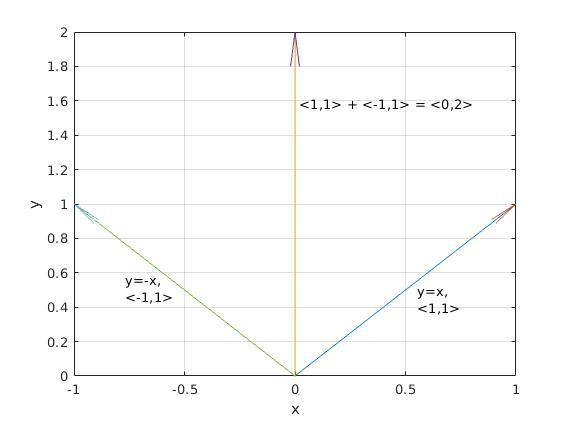
\includegraphics[width=\linewidth]{resources/img/not_closed_under_addition.png}
	 \caption{The blue arrows are vectors whose scalar multiples will all be in the same line as the blue arrows but the red arrow shows what happens if we add them; the result lies outside of both lines.}
	\end{figure}
	}
	
	\searchable{subsubsection}{Is $\R{2}$ a subspace of the complex vector space $\C{2}$?}{vector problems}{	
	The definition of a subspace of $\C{2}$ is a set of vectors which is a subset of those in $\C{2}$ and that forms a vector space under the same addition and scalar multiplication of $\C{2}$. The scalar multiplication of the vector space $\C{2}$ is multiplication by scalars $\lambda \in \C{}$.\\
	For a vector, $\v \in \R{2}$, scaling it by a complex number, $\lambda\v$ will result in a vector that is not necessarily in $\R{2}$.
	}
	
	\searchable{subsubsection}{Is $\setc{(a,b,c) \in \C{3}}{a^3 = b^3}$ a subspace of $\C{3}$?}{vector problems}{
	For $x \in \C{}$, $x^3$ has roots, $1, \frac{-1 + \sqrt{3}i}{2}, \frac{-1 - \sqrt{3}i}{2}$ so we don't have $a = b$ as we would if we were ranging over the reals. \\
	Concretely, we can have, $(1,\frac{-1 + \sqrt{3}i}{2},0)$ and $(1,\frac{-1 - \sqrt{3}i}{2},0)$ but,
	\[ (1,\frac{-1 + \sqrt{3}i}{2},0) + (1,\frac{-1 - \sqrt{3}i}{2},0) = (2,-1,0) \]
	where $(2,-1,0) \not\in \setc{(a,b,c) \in \C{3}}{a^3 = b^3}$ meaning that addition over this set is not closed. Therefore, this is not a subspace.
	}
	
	\searchable{subsubsection}{\small{Give an example of a non-empty subset $U$ of $\R{2}$ such that $U$ is closed under addition and under taking additive inverses (meaning $-\u \in U$ whenever $\u \in U$), but $U$ is not a subspace of $\R{2}$.}}{vector problems}{
	First thought might be $\R{2} - \{\0\}$ but this is \wrong. If the subset is closed under addition and under taking additive inverses then it means that $\u + -\u = \0 \in U$ and so the set $\R{2} - \{\0\}$ is not closed under addition and taking additive inverses.\\
	The set $\setc{(x,y) \in \R{2}}{x,y \in \Z{}}$ however, is closed under addition because integer addition is closed and under taking additive inverses but scalar multiplication where the scalars range over the reals, will produce non-integer values for $x$ and $y$.
	}
	
	\searchable{subsubsection}{\small{Is the set of periodic functions over the reals a subspace of $\R{R}$?}}{vector problems, periodic functions}{
	The definition of two periodic functions over the reals is
		\begin{align*}		
		\exists p > 0 \in \R{} \cdot f(x) &= f(x + p) \\
		\exists q > 0 \in \R{} \cdot g(x) &= g(x + q) \\
		\end{align*}
	Then for their sum to be periodic we need,
		\begin{align*}
		\exists \alpha, \beta \in \Z{}, m \in \R{} \cdot (m &= \alpha{p}) \wedge (m = \beta{q}) \\[7pt]
		\iff \frac{q}{p} &= \frac{\alpha}{\beta} \in \Q{} \\[7pt]
		\therefore (f + g)(x) = (f + g)(x + m) &= f(x + m) + g(x + m) \\[7pt]
		\iff \frac{q}{p} &\in \Q{}.
		\end{align*}
	}

	\searchable{subsubsection}{\small{Prove that the union of two subspaces of $V$ is a subspace of $V$ if and only if one of the subspaces is contained within the other.}}{vector problems}{
		Let $A, B$ be subspaces of $V$ and $\V{a} \in A,\; \V{b} \in B$ and, 
			\[ C = A \cup B = \setc{\V{c}}{\V{c} \in A \;\vee\; \V{c} \in B}. \]
		Since $\V{a},\V{b} \in C$ we have $\text{(C subspace of V)} \iff \forall\alpha,\beta \in F \,\cdot\, (\alpha\V{a} + \beta\V{b}) \in C$. Then,
		\begin{align*}
		\V{b} \in A &\implies \forall\alpha,\beta \in F \,\cdot\, (\alpha\V{a} + \beta\V{b}) \in A \sidecomment{ (by subspace properties) }\\
		&\implies (\alpha\V{a} + \beta\V{b}) \in C.
		\end{align*}
		A similar argument holds for $\V{a} \in B$. Conversely,
		\begin{align*}
		\forall\alpha,\beta \in F \,\cdot\, (\alpha\V{a} + \beta\V{b}) \in C &\implies ((\alpha\V{a} + \beta\V{b}) \in A) \vee ((\alpha\V{a} + \beta\V{b}) \in B)\\
		&\implies ((\alpha\V{a} - \alpha\V{a} + \beta\V{b}) = \beta\V{b} \in A) \vee ((\alpha\V{a} + \beta\V{b} - \beta\V{b}) = \alpha\V{a} \in B)\\
		&\implies (\V{b} \in A) \vee (\V{a} \in B)
		\end{align*}
		\begin{align*}
		\therefore \text{(C subspace of V)} &\iff \forall\alpha,\beta \in F \,\cdot\, (\alpha\V{a} + \beta\V{b}) \in C\\
		&\iff (\V{b} \in A) \vee (\V{a} \in B)\\
		&\equiv (B \subseteq A) \vee (A \subseteq B).
		\end{align*}
	}
	
	\searchable{subsubsection}{\small{Can a vector space over an infinite field be a finite union of proper subspaces?}}{vector problems}{
		Assume that our vector space V is a finite union of proper subspaces, hence
		\[ V=\bigcup_{i=1}^n U_i. \]
		Now, pick a non-zero vector $ \V{x} \in U_1 $, and pick another vector $ \V{y} \in V\,\backslash U_1. $\\
		
		There are infinitely many vectors $ \V{x} + k\V{y} $, where $ k\in K^* $ ($ K $ is our infinite field). Note that $ \V{x} + k\V{y} $ is not in $ U_1 $, hence must be contained in some $ U_j $ where $ j\neq 1 $.\\
		
		Then since $ k\in K^* $, we can have $ \V{x} + k_1\V{y},\, \V{x} + k_2\V{y} \in U_j $, which implies that it also contains $ \V{y} $ and hence also $ \V{x} $, hence $ U_1\subset U_j $.\\
		
		\textit{Explanation}: There are infinitely many vectors $\V{x} + k\V{y}$ and only finitely many $U_i$ so they cannot all be in different $U_i$ so we have,
		\begin{align*}
		\exists \, k_1,\, k_2 \in K^* \,\cdot\,  \V{x} + k_1\V{y},\, \V{x} + k_2\V{y} \in U_j \\
		\implies (\V{x} + k_1\V{y}) - (\V{x} + k_2\V{y}) = (k_1 - k_2)\V{y} \in U_j \\
		\implies \V{y} \in U_j \implies \V{x} \in U_j
		\end{align*}
		
		Hence
		\[ V=\bigcup_{i=2}^n U_i. \]
		
		Evidently, this can be continued, hence a contradiction arises.\\
	}
	
	\searchable{subsubsection}{\small{Prove or give a counterexample: if $U_1, U_2, W$ are subspaces of $V$ such that $ V = U_1 \oplus W \text{ and } V = U_2 \oplus W $ then $U_1 = U_2$.}}{vector problems}{
		Counter example: $V = \F{2}, \; U_1 = \setc{(x, 0) \in \F{2}}{x \in F}, \; U_2 = \setc{(0, x) \in \F{2}}{x \in F}, \; W = \setc{(x, x) \in \F{2}}{x \in F}$.	
	}
	
	\bigskip
	\searchable{subsubsection}{\small{Let $U_e$ denote the set of real-valued even functions on $\R{}$ and let $U_o$ denote the set of real-valued odd functions on $\R{}$. Show that $\R{R} = U_e \oplus U_o.$}}{vector problems}{
		Every function $f \in \R{R}$ can be expressed as the sum of an even function and an odd function as,
		\[ f(x) = \frac{f(x) + f(-x)}{2} + \frac{f(x) - f(-x)}{2} = g(x) + h(x) \]
	where $g(x) \in U_e$ and $h(x) \in U_o$. So, $U_e + U_o$ spans $\R{R}$.\\
	Furthermore,
	\begin{align*}
	f(x) \in (U_e \cap U_o) &\implies (f(-x) = f(x)) \wedge (f(-x) = -f(x))\\
	&\implies f(x) = -f(x)\\
	&\implies f(x) = 0
	\end{align*}
	Since $f(x) = 0$ is the additive identity of this space, this shows that the intersection is $ \0 $. So, $\R{R} = U_e \oplus U_o.$
	}


	
\bigskip\bigskip\bigskip\bigskip
\searchableSubsection{\sectionTitle{Span, Dimension and Bases}}{vector spaces}{\bigskip}
	
	\begin{definition}
	The \emph{span} of a list of vectors $\V{v_1}, \V{v_2}, \dots , \V{v_k}$ - written \emph{span$(\V{v_1}, \V{v_2}, \dots , \V{v_k})$} - is defined as
	\[ \setc{\alpha{_1}\V{v_1} + \alpha{_2}\V{v_2} + \dots + \alpha{_k}\V{v_k}}{\alpha{_1}, \alpha{_2}, \dots , \alpha{_k} \in F} \]
	\end{definition}
	
	\bigskip
	\labeledProposition{The span of a list of vectors is the smallest subspace containing those vectors.}{span_smallest_subspace}
	Note that a vector space over $\R{}$ or $\C{}$ is an uncountable set as - while the dimensions of the vector space may be finite - closure under scalar multiplication means that the vectors in the space are continuously valued as the field providing the scalars is continuously valued.\\
	This means that the notion of the \emph{smallest} subspace cannot refer to the cardinality of the set and must refer to ordering based on subset. So, the smallest subspace containing a list of vectors is a subspace that contains the list of vectors and, of which, there is no proper subset which also contains the list of vectors.	
	\begin{proof}
		\begin{align*}
		\text{Let } S &:= span(\V{v_1}, \V{v_2}, \dots , \V{v_k})\\
		 &:= \setc{\alpha{_1}\V{v_1} + \alpha{_2}\V{v_2} + \dots + \alpha{_k}\V{v_k}}{\alpha{_1}, \alpha{_2}, \dots , \alpha{_k} \in F}\\
		\text{and let }V &:= \text{ the smallest vector space containing }\V{v_1}, \V{v_2}, \dots , \V{v_k}.	 
		\end{align*}
		then $S$ contains every linear combination of $\V{v_1}, \V{v_2}, \dots , \V{v_k}$ and nothing else and so is a vector space containing $\V{v_1}, \V{v_2}, \dots , \V{v_k},$\\
		\[ V \subseteq S \]
		Additionally, any vector space containing the vectors $\V{v_1}, \V{v_2}, \dots , \V{v_k}$ must contain all their linear combinations, $span(\V{v_1}, \V{v_2}, \dots , \V{v_k}),$\\
		\[ S \subseteq V \]
		Therefore there is no proper subset of $span(\V{v_1}, \V{v_2}, \dots , \V{v_k})$ that is also a vector space containing $\V{v_1}, \V{v_2}, \dots , \V{v_k},$ and so $span(\V{v_1}, \V{v_2}, \dots , \V{v_k})$ is the smallest vector space containing $\V{v_1}, \V{v_2}, \dots , \V{v_k},$\\
		\[ (V \subseteq S) \wedge (S \subseteq V) \iff V = S \qedhere \]
	\end{proof}
	
	\bigskip
	\labeledProposition{Length of every linearly independent list in a space is less than or equal to the length of a spanning list in the same space.}{independent_list_smaller_than_spanning_list}
	\begin{proof}
	Let $U = \V{u_1}, \V{u_2}, \dots, \V{u_m}$ be a linearly independent list of vectors in $V$ and $W = \V{w_1}, \V{w_2}, \dots, \V{w_n}$ be a spanning list of vectors in $V$.\\
	If we take $\V{u_1}$ from $U$ and add it to $W$ then - since the other vectors in $W$ are a spanning list - $W$ must be linearly dependent. That's to say,
	\begin{align*}
	\exists\,\alpha_1,\alpha_2,\dots,\alpha_n \in \R{} \dotsuchthat &\alpha_1\V{w_1} + \dots + \alpha_n\V{w_n} = \V{u_1} \\[4pt]
	\iff &\alpha_1\V{w_1} + \dots + \alpha_n\V{w_n} - \V{u_1} = -\alpha_i\V{w_i}\\[4pt]
	\iff &\frac{-\alpha_1}{\alpha_i}\V{w_1} + \dots + \frac{-\alpha_n}{\alpha_i}\V{w_n} + \frac{1}{\alpha_i}\V{u_1} = \V{w_i}
	\end{align*}
	So, $\V{w_i}$ is in the span of $\V{u_1}, \V{w_2}, \dots, \V{w_n}$ and we can drop $\V{w_i}$ from the list, $W$, and it will still span the vector space.\\
	We can keep doing this with the remaining vectors in $U$ - each time the vector to be removed will be some $\V{w_i}$ because all the $\V{u_i}$ are linearly independent - and all the while $W$ remains a spanning list. We continue until we have replaced (potentially) all $n$ vectors in $W$, which would happen if $m > n$. At this point we would have the spanning list $W = \V{u_1}, \V{u_2}, \dots, \V{u_n}$ and $(m - n)$ remaining vectors in $U$.\\
	Now, since $W$ spans the space, the $(m - n)$ vectors that remain in $U$ will be in the span of $W$. But, all the vectors that originally came from $U$ were linearly independent, so it is impossible for any vectors in $U$ to be in the span of $W$ (which now comprises only vectors that originally came from $U$).\\
	We therefore conclude that there can be no remaining vectors in $U$ and, consequently that $m$ cannot be greater than $n$, i.e. $m \leq n$.
	\end{proof}
\end{document}